% Provenance (never printed): see sources/outline_sources.md (Year 3:
% sequence stratigraphy, accommodation and supply, systems tracts,
% cyclostratigraphy). Brief: sources/book5/BRIEFS.md, ch. 16. Curves from
% figdata/bachelor-3/shelf_model.py and lr04_periodogram.py. Exercise and
% problem values in the Book 5 scratch calculator calc/ch16.py. The Varden
% basin, its shelf and its core are invented.
\chapter{الستراتيغرافيا التتابعية}\label{ch:b3:sequence-stratigraphy}

عبر مقطع زلزالي لهامش قاري، تتراكب العواكس فوق ما هو أقدم منها،
ثم تمتدّ نحو الحوض، ثم تتراجع نحو اليابسة، ويتكرّر
النمط في الأعلى. تسجّل كلّ حزمة تنافسًا بين
معدّلين: معدّل تكوّن الحيّز المتاح للرواسب بفعل الهبوط وارتفاع البحر،
ومعدّل امتلاء هذا الحيّز بالأنهار. تقرأ الستراتيغرافيا
التتابعية هذا التنافس من هندسة الطبقات، \omterm{def:b3:sequence-stratigraphy:cyclo}{والستراتيغرافيا
الدورية} تقرأ ساعته من سماكتها.

\begin{recall}
الحيّز المتاح، والأيوستازيا، ومستوى البحر النسبي، والهبوط، والحوض الرسوبي،
موجودة في مجلد السنة الأولى، في فصله عن التحوّل بعد الترسيب والأحواض الرسوبية.
التجاوز البحري والانحسار البحري ودورة مستوى البحر من الرتبة الأولى
موجودة في مجلد السنة الثانية، في فصله عن الأرض الفانيروزية؛
ومعاملات ميلانكوفيتش والتقدّم المناخي في فصله عن القسر المداري
والعصور الجليدية؛ ونموذج العمر في فصله عن أرشيفات المناخ
والمؤشّرات البديلة. \omterm{def:b3:exploration-seismology:terminations}{التراكب الصاعد} \omterm{def:b3:exploration-seismology:terminations}{والتراكب الهابط} \omterm{def:b3:exploration-seismology:terminations}{والتراكب القمّي} \omterm{def:b3:exploration-seismology:terminations}{والبتر الحتّي} \omterm{def:b3:exploration-seismology:seismic-stratigraphy}{والستراتيغرافيا
الزلزالية} موجودة في الفصل~\ref{ch:b3:exploration-seismology}. متسلسلات فورييه
وتحويل فورييه موجودان في كتب الرياضيات.
\end{recall}

\section{الحيّز المتاح والإمداد وخط الشاطئ}\label{sec:b3:sequence-stratigraphy:shoreline}

عند أيّ نقطة من الحوض يرتفع مستوى البحر النسبي بالمعدّل $A = \dot E
+ \sigma$، أي المعدّل الأيوستاتي مضافًا إليه معدّل الهبوط (ويكون انخفاضًا عندما $A < 0$).
يتحدّد مستوى البحر النسبي عند موقع ما بمستوى سطح البحر العالمي وبكلّ
ما يحرّك اليابسة تحته: \omterm{def:b3:lithosphere-thermal-models:thermal-subsidence}{الهبوط الحراري}، وحمل
الرواسب والانثناء الذي يُحدثه، وارتداد القشرة بعد أن يذوب الغطاء
الجليدي، والدفع البطيء للوشاح تحت الصفيحة. ويُنشئ ارتفاعُ
مستوى البحر النسبي الحيّزَ المتاح، وتملؤه الرواسب. وما إذا كان
خط الشاطئ يتقدّم نحو البحر أو يتراجع نحو اليابسة يتوقّف على الأمرين معًا، لا على مستوى البحر
وحده.
% ledger: miller20:rsl

\begin{definition}[الانحسار العادي والانحسار القسري]\label{def:b3:sequence-stratigraphy:regression}
\emph{الانحسار العادي}\index{الانحسار العادي} هو تحرّك خط الشاطئ نحو البحر
بينما يرتفع مستوى البحر النسبي، إذ يفوق الإمداد
الحيّز المتاح المتكوّن عند خط الشاطئ. أمّا \emph{الانحسار القسري}\index{الانحسار القسري}
هو تحرّك نحو البحر يدفعه انخفاض مستوى البحر النسبي:
يُدفع خط الشاطئ نحو الحوض أيًّا كان الإمداد، وتتعرّض اليابسة التي تُترك خلفه
للانكشاف والتعرية.
\end{definition}

\begin{definition}[مسار خط الشاطئ]\label{def:b3:sequence-stratigraphy:trajectory}
\emph{مسار خط الشاطئ}\index{مسار خط الشاطئ} هو المسار الذي يسلكه خط الشاطئ
عبر الزمن، ويُرسم في مقطع الانحدار ضمن إطار
الرواسب، بحيث يُظهر الحركة الأفقية لخط الشاطئ وارتفاعه
أو انخفاضه بالنسبة إلى الطبقات السفلى.
\end{definition}

يجعل مقطعٌ بسيطٌ التنافسَ دقيقًا. خلف خط الشاطئ تقع الطبقات القمّية
المستوية عرضها $W$ عند مستوى البحر؛ وأمامها طبقات أمامية ميلها
$\tan\theta$ تنحدر حتى قاع الحوض، على ارتفاع $D$ تحتها.
ويمثّل الإمداد الرسوبي $Q$ حجمًا في وحدة الزمن لكلّ متر من الساحل (مساحة في وحدة
الزمن في المقطع).

\begin{proposition}[مسار خط الشاطئ]\label{prop:b3:sequence-stratigraphy:trajectory}
إذا ارتفع مستوى البحر النسبي ($A \ge 0$) وتراكمت الطبقات القمّية بانتظام،
يتحرّك خط الشاطئ بالمعدّل
\[
\frac{\mathrm dx_s}{\mathrm dt} = \frac{Q - AW}{D};
\]
ويتقدّم ما دام $Q > AW$، ويتراجع عندما $AW > Q$. وإذا كان مستوى البحر النسبي
ينخفض ($A < 0$)، فإنّ الطبقات القمّية لا تتلقّى شيئًا، ويكون
\[
\frac{\mathrm dx_s}{\mathrm dt} = \frac{Q}{D} + \frac{|A|}{\tan\theta}.
\]
في الحالتين يصعد المسار أو يهبط بالزاوية التي يكون ظلّها
$A/(\mathrm dx_s/\mathrm dt)$.
\end{proposition}

\begin{proof}
في زمن $\mathrm dt$ تحتاج الطبقات القمّية إلى $AW\,\mathrm dt$ من الرواسب كي تبقى
عند مستوى البحر. والباقي، $(Q - AW)\,\mathrm dt$، يُوزَّع على الطبقات الأمامية،
وهي جدار ارتفاعه $D$، فيتقدّم بمقدار $(Q - AW)\,\mathrm dt/D$؛ والباقي السالب
يعني أنّ البحر يغمر الطبقات القمّية أسرع مما تمتلئ به.
عندما ينخفض البحر، تكون الطبقات القمّية فوق الماء ولا تتلقّى شيئًا، وينزلق خط الشاطئ
نزولًا على الطبقات الأمامية القديمة بمقدار $|A|\,\mathrm dt/\tan\theta$ دون أيّ
رواسب، بينما يبني الإمداد كلّه الطبقات الأمامية إلى الأمام بمقدار $Q\,\mathrm
dt/D$. يرتفع خط الشاطئ بمقدار $A\,\mathrm dt$ بالنسبة إلى الطبقات السفلى
بينما يتحرّك بمقدار $\mathrm dx_s$، وهذا ما يحدّد الزاوية.
\end{proof}

ومنه يحتاج \omterm{def:b3:sequence-stratigraphy:regression}{الانحسار العادي} إلى إمداد أكبر من الحيّز المتاح
المتكوّن على الطبقات القمّية، ويصعد مساره؛ أمّا \omterm{def:b3:sequence-stratigraphy:regression}{الانحسار القسري} فيحدث
أيًّا كان الإمداد، ويهبط مساره. ونسبةُ المعدّلين،
ويُكتب غالبًا $A/S$، وتصنّف الأنماط: يحدث التقدّم عندما $A/S < 1$ على
الطبقات القمّية، والتراكم قرب 1، والتراجع فوقه.
ولذلك يمكن لمنحنى مستوى البحر نفسه أن يعطي انحسارًا على هامش غني بالرواسب،
وتجاوزًا بحريًّا على هامش فقير بها.

\section{الهندسة الطبقية: المتتاليات ومسالك الأنظمة}\label{sec:b3:sequence-stratigraphy:sequences}

انقطاعات العواكس الواردة في الفصل~\ref{ch:b3:exploration-seismology}
هي مفردات المنهج: يحدّد \omterm{def:b3:exploration-seismology:terminations}{التراكب الصاعد} \omterm{def:b3:exploration-seismology:terminations}{والتراكب الهابط} قاعدة
الحزمة، ويحدّد \omterm{def:b3:exploration-seismology:terminations}{التراكب القمّي} \omterm{def:b3:exploration-seismology:terminations}{والبتر الحتّي} قمّتها. وعند قراءتها في مقطع الانحدار،
تقسم الهامش إلى حزم محدّدة بأسطح لا ترسيب فيها أو
تعرية، تسجّل كلّ منها دورة واحدة من مستوى البحر النسبي.

\begin{definition}[المتتالية الترسيبية وحدّ المتتالية]\label{def:b3:sequence-stratigraphy:sequence}
\emph{المتتالية الترسيبية}\index{المتتالية الترسيبية} هي تتابع
من الطبقات المترابطة في نشأتها، دون انقطاع كبير داخلها، ومحدّدة عند قاعدتها
وقمّتها بعدم التوافق أو بالتوافقات التي تستمرّ عنها نحو
الحوض. وسطحها المحدِّد هو \emph{حدّ
المتتالية}\index{حدّ المتتالية}: عدم توافق يقطعه الانكشاف والتعرية
على الرصيف أثناء انخفاض مستوى البحر النسبي، ويمتدّ نحو الحوض
ليصير توافقًا مكافئًا.
\end{definition}

\begin{definition}[مسلك الأنظمة]\label{def:b3:sequence-stratigraphy:tract}
\emph{مسلك الأنظمة}\index{مسلك الأنظمة} هو مجموعة الأنظمة الترسيبية
(النهري، الساحلي، الرصيف، المنحدر) التي كانت نشطة معًا خلال جزء واحد
من دورة مستوى البحر النسبي، ويُتعرَّف عليها من موقعها في
المتتالية، ومن أسطحها المحدِّدة ونمط تكدّسها. ويُميَّز منها أربعة
هي:
\begin{itemize}
\item \emph{مسلك أنظمة طور الانخفاض}\index{مسلك أنظمة طور الانخفاض}،
  يُبنى \omterm{def:b3:sequence-stratigraphy:regression}{بالانحسار القسري} بينما ينخفض مستوى البحر النسبي:
  الطبقات الأمامية المتدرّجة نحو الأسفل المنفصلة عن الرصيف القديم؛
\item \emph{مسلك أنظمة المستوى المنخفض}\index{مسلك أنظمة المستوى المنخفض}،
  يُبنى \omterm{def:b3:sequence-stratigraphy:regression}{بالانحسار العادي} حين يبدأ مستوى البحر النسبي بالارتفاع من جديد،
  عند أدنى موقع لخط الشاطئ: إسفين يتراكم رأسيًا ويتقدّم نحو الحوض؛
\item \emph{مسلك الأنظمة التجاوزي}\index{مسلك الأنظمة التجاوزي}،
  يُبنى أثناء تراجع خط الشاطئ نحو اليابسة: وحدات متراجعة التدرّج
  تُظهر تراكبًا صاعدًا على الرصيف القديم؛
\item \emph{مسلك أنظمة المستوى المرتفع}\index{مسلك أنظمة المستوى المرتفع}،
  يُبنى \omterm{def:b3:sequence-stratigraphy:regression}{بالانحسار العادي} في نهاية الارتفاع، حين يعود الإمداد فيفوق
  الحيّز المتاح للترسيب: طبقات أمامية تتقدّم نحو الحوض، وتُظهر تراكبًا هابطًا على الرواسب الواقعة تحتها.
\end{itemize}
\end{definition}

\begin{definition}[السطح التجاوزي وسطح الغمر الأقصى]\label{def:b3:sequence-stratigraphy:surfaces}
\emph{السطح التجاوزي}\index{السطح التجاوزي} هو أوّل سطح غمر مهمّ يعلو
رواسب المستوى المنخفض، وهو يُعلِّم
تحوّل خط الشاطئ من الانحسار إلى التجاوز. ويمثّل \emph{سطح الغمر
الأقصى}\index{سطح الغمر الأقصى} يحدّد أبعد موضع يبلغه خط
الشاطئ نحو اليابسة، وهو تحوّل من التجاوز إلى انحسار المستوى المرتفع؛ وتتراكب
الطبقات الأمامية للمستوى المرتفع تراكبًا هابطًا عليه.
\end{definition}

\begin{definition}[المقطع المكثَّف والوادي المحفور]\label{def:b3:sequence-stratigraphy:condensed}
\emph{المقطع المكثَّف}\index{المقطع المكثَّف} هو فترة رقيقة
تترسّب ببطء شديد بعيدًا عن خط الشاطئ بينما يغمر البحر الرصيف
ويُحتجز الرسوب قرب الساحل: بضعة سنتيمترات أو ديسيمترات
من الطين والأحافير والغلوكونيت أو الفوسفات، وقد تسجّل زمنًا طويلًا. أمّا
\emph{الوادي المحفور}\index{الوادي المحفور} هو وادٍ نهري محفور في
الرصيف المكشوف أثناء انخفاض مستوى البحر النسبي، ويُملأ خلال
مرحلتَي المستوى المنخفض والتجاوز اللاحقتين.
\end{definition}

\begin{omfigure}
\begin{tikzpicture}[font=\scriptsize, x=0.9cm, y=1.25cm, >=Stealth]
% older highstand deposits below the sequence boundary
\fill[black!10] (0,0) -- (14,0) -- (14,0.4) -- (10,0.6) -- (6,2.8) -- (0,3.0) -- cycle;
\draw[black!35] (1.5,2.0) .. controls (3.2,1.95) and (4.5,1.2) .. (8.5,0.45);
\draw[black!35] (3.5,2.93) .. controls (4.8,2.85) and (6,1.6) .. (10.5,0.42);
% falling-stage systems tract
\fill[red!25] (6.0,2.8) -- (7.4,2.25) -- (8.4,1.85) -- (9.4,1.35) -- (10.4,0.75) -- (10.6,0.58) -- (10,0.6) -- cycle;
\draw[red!60!black] (6.6,2.56) .. controls (7.0,2.4) and (7.5,1.95) .. (8.0,1.70);
\draw[red!60!black] (7.6,2.17) .. controls (8.0,2.0) and (8.5,1.45) .. (9.0,1.15);
\draw[red!60!black] (8.6,1.75) .. controls (9.0,1.55) and (9.5,0.9) .. (10.0,0.6);
% lowstand wedge
\fill[orange!40] (9.2,1.45) -- (10.4,1.5) -- (11.5,1.0) -- (12.6,0.6) -- (13.4,0.44) -- (10.6,0.58) -- (10.4,0.75) -- cycle;
% incised valley and its fill
\fill[orange!30] (2.9,2.9) .. controls (3.3,2.3) and (3.9,2.3) .. (4.3,2.86) -- cycle;
% transgressive systems tract
\fill[green!45!black!35] (11.5,1.0) -- (10.4,1.5) -- (9.2,1.45) -- (8.4,1.85) -- (7.4,2.25) -- (6.0,2.8) -- (1.0,2.97) -- (1.0,3.05) -- (6.0,2.95) -- (7.6,2.5) -- (9.4,1.75) -- (10.8,1.45) -- cycle;
% highstand systems tract
\fill[blue!22] (0,3.62) -- (7.5,3.42) -- (9.8,2.2) -- (11.2,1.22) -- (10.8,1.45) -- (9.4,1.75) -- (7.6,2.5) -- (6.0,2.95) -- (1.0,3.05) -- (0,3.07) -- cycle;
\draw[blue!60!black] (4.0,3.52) .. controls (5.0,3.45) and (5.8,3.1) .. (6.6,2.79);
\draw[blue!60!black] (5.6,3.47) .. controls (6.6,3.4) and (7.4,2.8) .. (8.2,2.26);
\draw[blue!60!black] (6.8,3.44) .. controls (7.8,3.35) and (8.8,2.4) .. (9.7,1.69);
% surfaces
\draw[red!70!black, very thick] (0,3.0) -- (2.9,2.9) .. controls (3.3,2.3) and (3.9,2.3) .. (4.3,2.86) -- (6.0,2.8) -- (7.4,2.25) -- (8.4,1.85) -- (9.2,1.45);
\draw[red!70!black, very thick, densely dashed] (9.2,1.45) -- (9.4,1.35) -- (10.4,0.75) -- (10.6,0.58) -- (14,0.4);
\draw[green!40!black, thick] (11.5,1.0) -- (10.4,1.5) -- (9.2,1.45);
\draw[blue!60!black, thick] (0,3.07) -- (1.0,3.05) -- (6.0,2.95) -- (7.6,2.5) -- (9.4,1.75) -- (10.8,1.45) -- (11.5,1.03) -- (12.6,0.63) -- (13.4,0.47) -- (14,0.43);
% labels
\node[blue!50!black] at (2.6,3.36) {\foreignlanguage{arabic}{المستوى المرتفع \mbox{\textdir TLT (HST)}}};
\node[green!35!black, anchor=south] at (4.8,3.92) {\foreignlanguage{arabic}{التجاوزي \mbox{\textdir TLT (TST)}}};
\draw[green!35!black] (4.8,3.92) -- (4.4,3.01);
\node[red!60!black, anchor=west] at (10.1,2.45) {\foreignlanguage{arabic}{طور الانخفاض \mbox{\textdir TLT (FSST)}}};
\draw[red!60!black] (10.1,2.45) -- (8.8,1.62);
\node[orange!60!black, anchor=west] at (12.2,1.55) {\foreignlanguage{arabic}{المستوى المنخفض \mbox{\textdir TLT (LST)}}};
\draw[orange!60!black] (12.2,1.55) -- (11.2,0.85);
\node[anchor=north, align=center] at (3.6,2.25) {الوادي\\ المحفور};
\node[red!70!black, anchor=north] at (1.4,2.95) {SB};
\node[red!70!black, anchor=north] at (12.0,0.38) {التوافق المكافئ};
\node[blue!60!black, anchor=west] at (12.7,1.1) {MFS};
\draw[blue!60!black] (12.7,1.1) -- (12.1,0.82);
\node[green!40!black, anchor=west] at (11.6,2.0) {TS};
\draw[green!40!black] (11.6,2.0) -- (10.9,1.27);
\node[blue!60!black, anchor=south] at (13.4,0.58) {مكثَّف};
\node[anchor=west, black!60] at (0.2,0.35) {رواسب أقدم};
\draw[->] (11.2,3.9) -- (12.6,3.9) node[right] {نحو الحوض};
\end{tikzpicture}

\par\smallskip{\small تشريح متتالية ترسيبية في مقطع الانحدار
(رسم تخطيطي، والمقياس الرأسي مبالغ فيه كثيرًا). \omterm{def:b3:sequence-stratigraphy:sequence}{وحدّ المتتالية} (SB، بالأحمر)
هو عدم توافق على الرصيف، مع وادٍ محفور، وتوافق مكافئ
في الحوض (متقطّع)؛ وهو مرسوم هنا فوق رواسب طور
الانخفاض. ويعلو \omterm{def:b3:sequence-stratigraphy:surfaces}{السطح التجاوزي} (TS) إسفين المستوى المنخفض؛ ويعلو \omterm{def:b3:sequence-stratigraphy:surfaces}{سطح الغمر الأقصى}
(MFS) المسلك التجاوزي الرقيق ويمتدّ نحو الحوض
ليصير مقطعًا مكثَّفًا؛ وتتراكب الطبقات الأمامية للمستوى المرتفع تراكبًا هابطًا عليه.}\label{fig:b3:sequence-stratigraphy:anatomy}
\end{omfigure}

تحديد موضع \omterm{def:b3:sequence-stratigraphy:sequence}{حدّ المتتالية} بالضبط في الحوض مسألة اصطلاحية،
والمؤلفون يختلفون فيه: فبعضهم يرسمه عند قاعدة رواسب طور الانخفاض، حيث
يبدأ الانخفاض، وبعضهم عند قمّتها حيث ينتهي، كما في الشكل أعلاه.
أمّا على الرصيف فلا لبس: فالحدّ هو سطح الانكشاف
والتعرية، والرواسب الواقعة فوقه أحدث من الانخفاض.

تُقرأ من الأسفل إلى الأعلى عند موضع واحد على الرصيف الخارجي، تسجّل المتتالية
الدورة: طبقات أمامية للمستوى المرتفع، وسطح انكشاف، وربما ملء وادٍ،
\omterm{def:b3:sequence-stratigraphy:surfaces}{السطح التجاوزي}، وطبقات متراجعة التدرّج، وفترة مكثَّفة عند
\omterm{def:b3:sequence-stratigraphy:surfaces}{سطح الغمر الأقصى}، ثم طبقات أمامية للمستوى المرتفع من جديد. وتتحدّد هرمية
الدورات بأسبابها: فتح المحيطات وإغلاقها للدورة من الرتبة الأولى،
تغيّرات حجم الجليد وسرعة
انتشار قاع البحر في الدورات الأقصر، والتكتونيات المحلية والإمداد لكلّ
منها.

\section{المتتاليات الفرعية وأنماط التكدّس}\label{sec:b3:sequence-stratigraphy:parasequences}

داخل \omterm{def:b3:sequence-stratigraphy:tract}{مسلك الأنظمة}، أصغر الحزم التي يرسمها الجيولوجي على جرف أو على سجلّ
بئر، هي وحدات تتضحّل نحو الأعلى، سماكتها من بضعة أمتار إلى بضع
عشرات من الأمتار، يعلوها سطح يعود عنده الماء العميق فجأةً.

\begin{definition}[المتتالية الفرعية وسطح الغمر]\label{def:b3:sequence-stratigraphy:parasequence}
\emph{المتتالية الفرعية}\index{المتتالية الفرعية} هي تتابع متوافق نسبيًّا
من طبقات مترابطة من حيث المنشأ، تحدّه أسطح الغمر، ويضحل فيه الماء نحو الأعلى:
على ساحل تسيطر عليه الأمواج، ينتقل الطين البحري المفتوح صعودًا
إلى رمال الوجه الشاطئي السفلي والعلوي والشاطئ. أمّا
\emph{سطح الغمر}\index{سطح الغمر} هو سطح تعلو عبره فجأة سحنات المياه الأعمق سحنات الأضحل،
مع دلائل على تعمّق مفاجئ.
\end{definition}

تخشن \omterm{def:b3:sequence-stratigraphy:parasequence}{المتتالية الفرعية} المفردة نحو الأعلى، ويأخذ سجلّ أشعة غاما لها،
المنخفض في الرمل والمرتفع في الطين، شكلًا قمعيًّا يضيق نحو الأعلى. وتدلّ طريقة تكدّس
المتتاليات الفرعية في المسلك بعضها فوق بعض على اتجاه
خط الشاطئ: فكلّ متتالية بُنيت أبعد نحو البحر من سابقتها (تقدّمية)،
أو فوقها تمامًا (تراكمية)، أو نحو اليابسة منها (تراجعية). ويُظهر سجلّ يمرّ
عبر التكدّس الاتجاه مباشرةً: تنتهي كلّ متتالية فرعية بسحنات أخشن وأضحل من التي تحتها،
أو مماثلة لها، أو أدقّ وأعمق.
تتكدّس مسالك المستوى المرتفع والمنخفض تقدّميًّا أو تراكميًّا،
أمّا مسالك الأنظمة التجاوزية فتتكدّس تراجعيًّا. ويقرأ الفصل التالي مثل هذه السجلّات
سحنةً سحنةً.

\begin{omfigure}
\begin{tikzpicture}[font=\scriptsize, x=1cm, y=1cm]
% three logs: each parasequence a coarsening-upward wedge (grain size to the right)
% progradational
\begin{scope}[xshift=0cm]
\fill[yellow!45!brown!35] (0,0) -- (0.5,0) -- (1.4,1.1) -- (0,1.1) -- cycle;
\fill[yellow!45!brown!35] (0,1.1) -- (0.5,1.1) -- (1.8,2.2) -- (0,2.2) -- cycle;
\fill[yellow!45!brown!35] (0,2.2) -- (0.5,2.2) -- (2.2,3.3) -- (0,3.3) -- cycle;
\draw (0,0) -- (0.5,0) -- (1.4,1.1) -- (0.5,1.1) -- (1.8,2.2) -- (0.5,2.2) -- (2.2,3.3) -- (0,3.3) -- cycle;
\node[anchor=north, align=center] at (1.1,-0.1) {تقدّمية\\ (يتحرّك خط الشاطئ نحو البحر)};
\end{scope}
% aggradational
\begin{scope}[xshift=4.2cm]
\fill[yellow!45!brown!35] (0,0) -- (0.5,0) -- (1.8,1.1) -- (0,1.1) -- cycle;
\fill[yellow!45!brown!35] (0,1.1) -- (0.5,1.1) -- (1.8,2.2) -- (0,2.2) -- cycle;
\fill[yellow!45!brown!35] (0,2.2) -- (0.5,2.2) -- (1.8,3.3) -- (0,3.3) -- cycle;
\draw (0,0) -- (0.5,0) -- (1.8,1.1) -- (0.5,1.1) -- (1.8,2.2) -- (0.5,2.2) -- (1.8,3.3) -- (0,3.3) -- cycle;
\node[anchor=north, align=center] at (1.1,-0.1) {تراكمية\\ (يبقى خط الشاطئ ثابتًا)};
\end{scope}
% retrogradational
\begin{scope}[xshift=8.4cm]
\fill[yellow!45!brown!35] (0,0) -- (0.5,0) -- (2.2,1.1) -- (0,1.1) -- cycle;
\fill[yellow!45!brown!35] (0,1.1) -- (0.5,1.1) -- (1.8,2.2) -- (0,2.2) -- cycle;
\fill[yellow!45!brown!35] (0,2.2) -- (0.5,2.2) -- (1.4,3.3) -- (0,3.3) -- cycle;
\draw (0,0) -- (0.5,0) -- (2.2,1.1) -- (0.5,1.1) -- (1.8,2.2) -- (0.5,2.2) -- (1.4,3.3) -- (0,3.3) -- cycle;
\node[anchor=north, align=center] at (1.1,-0.1) {تراجعية\\ (يتحرّك خط الشاطئ نحو اليابسة)};
\end{scope}
% flooding surfaces
\foreach \s in {0,4.2,8.4} {
  \draw[omDef, thick] (\s-0.15,1.1) -- (\s+2.5,1.1);
  \draw[omDef, thick] (\s-0.15,2.2) -- (\s+2.5,2.2);
  \node[omDef, anchor=west] at (\s+2.5,1.1) {FS};
  \node[omDef, anchor=west] at (\s+2.5,2.2) {FS};
}
% grain-size axis
\draw[->] (0,3.6) -- (2.3,3.6) node[right] {أخشن};
\node[anchor=east] at (0,3.6) {طين};
\end{tikzpicture}

\par\smallskip{\small ثلاث متتاليات فرعية مكدّسة بثلاث طرق، مرسومة
في صورة سجلّات لحجم الحبيبات (العرض نحو اليمين يعني أخشن). تتخشّن كلّ
متتالية فرعية نحو الأعلى من الطين البحري المفتوح إلى رمل الوجه الشاطئي،
وتنتهي بسطح غمر (FS)؛ وتكون قمّة كلّ منها أخشن من التي تحتها عندما يتقدّم التكدّس،
ومماثلة لها عندما يتراكم، وأدقّ عندما
يتراجع.}\label{fig:b3:sequence-stratigraphy:stacking}
\end{omfigure}

\begin{inthefield}[المتتاليات الفرعية في جرف صحراوي]
\begin{minipage}[t]{0.52\linewidth}\vspace{0pt}
تكشف جروف بوك في شرق يوتا ترسّبات خط شاطئ من الكريتاسي الأعلى
لعشرات الكيلومترات. وفي عضو كينيلوورث، المتتبَّع على امتداد الجروف
من برايس إلى هاتش ميسا، رسم الجيولوجيّون ترسّبات السهل الساحلي والوجه الشاطئي،
والرصيف الداخلي وترسّبات \omterm{def:b3:sequence-stratigraphy:condensed}{الوادي المحفور}، وتسع متتاليات فرعية تتخشّن نحو الأعلى،
تهيمن عليها الأمواج إلى العواصف، سماكتها من 7 إلى \qty{32}{m}. وتتفرّع نحو الحوض
كلّ منها إلى ما يصل إلى أربع مجموعات طبقية أصغر تتخشّن نحو الأعلى، سماكتها من 2 إلى
\qty{18}{m}؛ وتستقرّ بعض رمال الوجه الشاطئي على قاعدة حادّة، تعدّها الدراسة
ترسّبات المستوى المنخفض.
\end{minipage}\hfill
\begin{minipage}[t]{0.44\linewidth}\vspace{0pt}
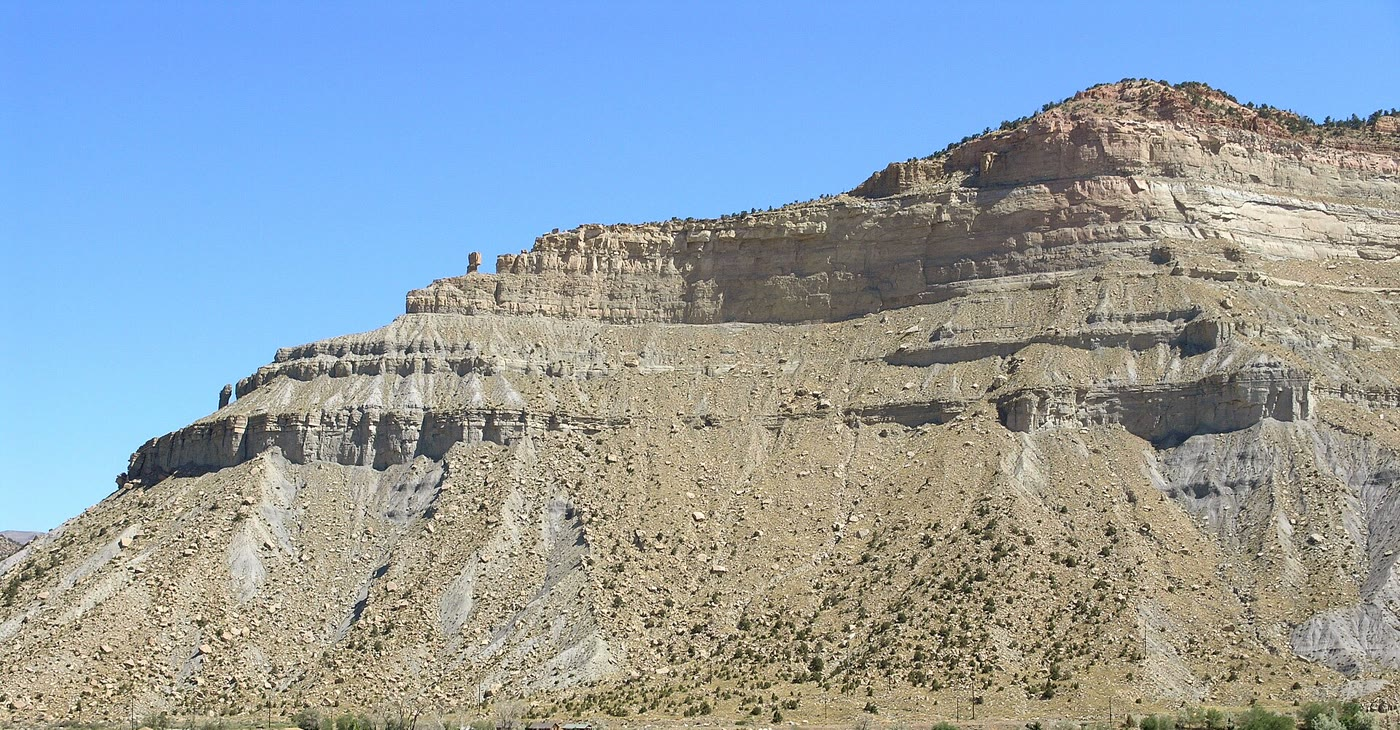
\includegraphics[width=\linewidth]{images/book5/b3-book-cliffs-helper.jpg}

{\scriptsize جروف بوك فوق هيلبر في يوتا: حافّات من الحجر الرملي الفاتح تبرز
فوق منحدرات من الحجر الطيني الرمادي. الصورة: \mbox{\textdir TLT David Mackie}، ملك عام.}
\end{minipage}
\end{inthefield}
% ledger: pattison95:kenilworth, photo:b3-book-cliffs

\section{نموذج أمامي للرصيف}\label{sec:b3:sequence-stratigraphy:model}

يمكن تشغيل القواعد الواردة في الأقسام السابقة في صورة نموذج. حوض فاردن
هو رصيف متخيَّل: منحدر يميل نحو الحوض بمقدار \qty{1.5}{m/km}، ويهبط
بمعدّل $\sigma = 0.02 + x/1200$ \unit{m/kyr} عند مسافة $x$ \babelsublr{(km)} من
المفصل، تحت مستوى سطح البحر $E = -30\cos(2\pi t/400)$ (\unit{m}، $t$ بوحدة \unit{kyr})، يغذّيه نهر
يمدّه بمقدار $Q = \qty{6000}{m^3/kyr}$ لكلّ متر من الساحل. وفي كلّ خطوة
من خطوات نصف ألف سنة يهبط الحوض؛ ثم تملأ الرواسب سطحًا علويًّا
مستويًا حتى مستوى سطح البحر حيثما كان السطح القديم تحت الماء، وطبقات أمامية
بميل 0.012 أمامه، ويُوضع خط الشاطئ بحيث يساوي الحجم المضاف
الإمداد؛ ولا تستقبل اليابسة المكشوفة شيئًا، وهي، للتبسيط،
غير معرّضة للتعرية. ويبدأ النموذج عند المستوى المنخفض، بعد إسفين أوّل
بُني عند مستوى سطح بحر ثابت.

\begin{omfigure}
\begin{tikzpicture}
\begin{groupplot}[group style={group size=1 by 2, vertical sep=0.35cm, x descriptions at=edge bottom},
  omrecord, width=0.86\linewidth, xmin=0, xmax=600,
  xtick={0,100,200,300,400,500,600},
  tick label style={font=\scriptsize}, label style={font=\small}]
\nextgroupplot[height=0.2\linewidth, ylabel={مستوى سطح البحر $E$ \babelsublr{(\unit{m})}}, ymin=-35, ymax=35,
  ytick={-30,0,30}]
\addplot[omDef, thick, domain=0:600, samples=121] {-30*cos(deg(2*pi*x/400))};
\nextgroupplot[height=0.3\linewidth, xlabel={الزمن \babelsublr{(\unit{kyr})}}, ylabel={خط الشاطئ $x_s$ \babelsublr{(km)}},
  ymin=0, ymax=60, ytick={0,20,40,60},
  scatter/classes={1={mark=*, red!70!black}, 2={mark=*, orange!80!black},
    3={mark=*, green!50!black}, 4={mark=*, blue!70!black}}]
% computed in figdata/bachelor-3/shelf_model.py
\addplot[scatter, only marks, mark size=0.9pt, scatter src=explicit symbolic]
  table[x=t, y=xs, meta=tract] {figdata/out/bachelor-3-shelf_model-shore.dat};
\node[font=\scriptsize, orange!60!black] at (axis cs:12,56) {LST};
\node[font=\scriptsize, green!40!black] at (axis cs:70,40) {TST};
\node[font=\scriptsize, blue!60!black] at (axis cs:160,6) {HST};
\node[font=\scriptsize, red!60!black] at (axis cs:300,22) {FSST};
\node[font=\scriptsize, orange!60!black] at (axis cs:415,57) {LST};
\node[font=\scriptsize, green!40!black] at (axis cs:520,45) {TST};
\node[font=\scriptsize, blue!60!black] at (axis cs:580,12) {HST};
\end{groupplot}
\end{tikzpicture}

\par\smallskip{\small في الأعلى، مستوى سطح البحر الأوستاتيكي لنموذج فاردن؛
وفي الأسفل، موضع خط الشاطئ، ملوَّنًا بحسب \omterm{def:b3:sequence-stratigraphy:tract}{مسلك الأنظمة} (المستوى المنخفض
البرتقالي، والتجاوزي الأخضر، والمستوى المرتفع الأزرق، وطور الانخفاض الأحمر)، مصنَّفًا
من مخرجات النموذج وحدها: طور الانخفاض عندما ينخفض مستوى البحر النسبي
عند خط الشاطئ، والتجاوزي عندما يتراجع خط الشاطئ، والمستوى المنخفض أو
المرتفع عندما يتقدّم تحت بحرٍ صاعد، بعد انخفاض أو بعد
التجاوز البحري.}\label{fig:b3:sequence-stratigraphy:series}
\end{omfigure}

يتتبّع الشكل أعلاه خط الشاطئ عبر الزمن، أمّا الشكل أدناه
فيُظهر الرواسب التي خلّفها. وتظهر المسالك دون قاعدة مكتوبة في النموذج
سوى الملء والهبوط. يقع إسفين المستوى المنخفض في البداية بعيدًا
نحو الحوض؛ إذ يدفع البحر الصاعد خط الشاطئ \qty{38}{km} نحو اليابسة في
التجاوز الأول، وتبني الواجهات المائلة للمستوى المرتفع امتدادها من جديد مع تباطؤ الارتفاع.
ثم يبدأ الانخفاض: يُدفع خط الشاطئ نحو الحوض بمقدار \qty{33}{km} في
\qty{187}{kyr}، تاركًا واجهات مائلة رقيقة متدرّجة نحو الأسفل ورصيفًا مكشوفًا
خلفه، وهو مسلك طور الانخفاض. ويلي ذلك إسفين جديد للمستوى المنخفض، وتجاوز بحري ثانٍ
ومستوى مرتفع جديد. وتطابق سرعة \omterm{def:b3:sequence-stratigraphy:regression}{الانحسار القسري} في النموذج
صيغة القضية في حدود بضعة في المئة؛ وتحت بحر صاعد لا تتراكم
الواجهة العلوية للنموذج بانتظام، إذ يزداد الهبوط نحو الحوض،
والصيغة مجرّد دليل إرشادي.

\begin{omfigure}
\begin{tikzpicture}
\begin{axis}[omsection, width=0.95\linewidth, height=0.42\linewidth,
  xmin=0, xmax=70, ymin=-150, ymax=40, clip=true,
  xlabel={المسافة نحو الحوض (km)}, ylabel={الارتفاع الحالي (m)},
  xtick={0,10,20,30,40,50,60,70}, ytick={-150,-100,-50,0},
  tick label style={font=\scriptsize}, label style={font=\small}]
% computed in figdata/bachelor-3/shelf_model.py
\addplot[fill=black!10, draw=none] table[x=x, y=z0] {figdata/out/bachelor-3-shelf_model-surfaces.dat} -- (axis cs:120,-300) -- (axis cs:0,-300) -- cycle;
\addplot[fill=orange!45, draw=none] table[x=x, y=z] {figdata/out/bachelor-3-shelf_model-poly1.dat};
\addplot[fill=green!45!black!35, draw=none] table[x=x, y=z] {figdata/out/bachelor-3-shelf_model-poly2.dat};
\addplot[fill=blue!25, draw=none] table[x=x, y=z] {figdata/out/bachelor-3-shelf_model-poly3.dat};
\addplot[fill=red!30, draw=none] table[x=x, y=z] {figdata/out/bachelor-3-shelf_model-poly4.dat};
\addplot[fill=orange!45, draw=none] table[x=x, y=z] {figdata/out/bachelor-3-shelf_model-poly5.dat};
\addplot[fill=green!45!black!35, draw=none] table[x=x, y=z] {figdata/out/bachelor-3-shelf_model-poly6.dat};
\addplot[fill=blue!25, draw=none] table[x=x, y=z] {figdata/out/bachelor-3-shelf_model-poly7.dat};
\addplot[black!45, very thin] table[x=x, y=z40] {figdata/out/bachelor-3-shelf_model-surfaces.dat};
\addplot[black!45, very thin] table[x=x, y=z80] {figdata/out/bachelor-3-shelf_model-surfaces.dat};
\addplot[black!45, very thin] table[x=x, y=z120] {figdata/out/bachelor-3-shelf_model-surfaces.dat};
\addplot[black!45, very thin] table[x=x, y=z160] {figdata/out/bachelor-3-shelf_model-surfaces.dat};
\addplot[black!45, very thin] table[x=x, y=z240] {figdata/out/bachelor-3-shelf_model-surfaces.dat};
\addplot[black!45, very thin] table[x=x, y=z280] {figdata/out/bachelor-3-shelf_model-surfaces.dat};
\addplot[black!45, very thin] table[x=x, y=z320] {figdata/out/bachelor-3-shelf_model-surfaces.dat};
\addplot[black!45, very thin] table[x=x, y=z360] {figdata/out/bachelor-3-shelf_model-surfaces.dat};
\addplot[black!45, very thin] table[x=x, y=z440] {figdata/out/bachelor-3-shelf_model-surfaces.dat};
\addplot[black!45, very thin] table[x=x, y=z480] {figdata/out/bachelor-3-shelf_model-surfaces.dat};
\addplot[black!45, very thin] table[x=x, y=z520] {figdata/out/bachelor-3-shelf_model-surfaces.dat};
\addplot[black!45, very thin] table[x=x, y=z560] {figdata/out/bachelor-3-shelf_model-surfaces.dat};
\addplot[black, thin] table[x=x, y=z600] {figdata/out/bachelor-3-shelf_model-surfaces.dat};
\addplot[black, only marks, mark=*, mark size=0.5pt] table[x=xs, y=zfinal] {figdata/out/bachelor-3-shelf_model-shore.dat};
\node[font=\scriptsize, blue!50!black] at (axis cs:6,4) {HST};
\node[font=\scriptsize, green!30!black] at (axis cs:12,-22) {TST};
\node[font=\scriptsize, red!60!black] at (axis cs:35,-25) {FSST};
\node[font=\scriptsize, orange!60!black] at (axis cs:57.5,-60) {LST};
\node[font=\scriptsize, green!30!black] at (axis cs:36,2) {TST};
\node[font=\scriptsize, blue!50!black] at (axis cs:8,26) {HST};
\end{axis}
\end{tikzpicture}

\par\smallskip{\small الرصيف في فاردن بعد \qty{600}{kyr}، في موضعه الحالي
(مقياس رأسي مبالَغ فيه بنحو 170 مرة). وتمثّل الألوان
مسالك الأنظمة: المستوى المنخفض البرتقالي، والتجاوزي الأخضر، والمرتفع الأزرق،
وطور الانخفاض الأحمر؛ والرمادي هو المنحدر الأقدم والإسفين الأول. والخطوط الرفيعة
تمثّل قاع البحر كل \qty{40}{kyr}؛ والنقاط السوداء ترسم خط الشاطئ كل
\qty{2}{kyr}. محسوبة بالنموذج الأمامي الوارد في
النص.}\label{fig:b3:sequence-stratigraphy:section}
\end{omfigure}


يبدأ مستوى البحر النسبي بالانخفاض عند خط الشاطئ بعد بضعة آلاف من السنين
من المستوى المرتفع الأوستاتيكي، لأنّ الهبوط يجب أن يُتجاوَز أولًا،
وينتهي قبل المستوى المنخفض الأوستاتيكي بضعة آلاف من السنين.
ولذلك يدوم الانخفاض عند خط الشاطئ أقلّ من نصف الدورة الأوستاتيكية، ويكون ذلك أشدّ
كلّما هبط الحوض أسرع.

تُعدّ النماذج من هذا النوع الاختبار الصادق لأيّ تفسير، وتُظهر أيضًا
حدوده. ويمكن بناء المقطع نفسه بتواريخ مختلفة: انخفاض أسرع مع إمداد أقل،
أو انخفاض أبطأ مع إمداد أكبر، أو تغيّر في الهبوط لا في مستوى البحر،
إذ لا تسجّل الهندسة إلا مستوى البحر النسبي
والإمداد. وقد حدّدت المخططات العالمية لدورات مستوى البحر، المبنيّة على الهوامش القارية في عقدَي 1970 و1980،
توقيت كثير من الانخفاضات التي أكّدتها الحفريات إلى حدّ كبير منذ ذلك الحين
في أجزاء من الطباشيري المتأخّر حتى الميوسين، لكنّ سعاتها،
مثل انخفاض مقداره \qty{160}{m} في الأوليغوسين الأوسط، مبالَغ فيها بعامل من 2 إلى 3.
وتُؤخذ السعات الأوستاتيكية الآن من نظائر الأكسجين
ومن الآبار المُعاد بناؤها بإزالة الطبقات تباعًا، وتُقرأ المتتاليات الترسيبية للهامش
أوّلًا بوصفها سجلًّا محلّيًّا.
% ledger: miller20:epr, miller20:rsl

\section{الستراتيغرافيا الدورية}\label{sec:b3:sequence-stratigraphy:cyclo}

تتكرّر تتابعات رسوبية كثيرة عند فواصل سماكة منتظمة: أزواج
من المارل والحجر الجيري، وحُزم من خمسة أزواج، ومجموعات أكبر من الحُزم. وإذا
كان التكرار مضبوطًا بوسائط ميلانكوفيتش، تحوّلت سماكة الدورات
إلى زمن.

\begin{definition}[الستراتيغرافيا الدورية والمعايرة الفلكية]\label{def:b3:sequence-stratigraphy:cyclo}
\emph{الستراتيغرافيا الدورية}\index{الستراتيغرافيا الدورية} تُحدّد وتقيس
الدورات المنتظمة في التتابعات الرسوبية، وتفسّرها بوصفها سجلّات
لقسرٍ دوري، أهمّه تغيّرات مدار الأرض ومحورها.
\emph{المعايرة الفلكية}\index{المعايرة الفلكية} تُسند أعمارًا إلى تتابع
بمطابقة دوراته واحدةً واحدةً مع
سلسلة فلكية محسوبة (الاختلاف المركزي، والميل المحوري، والتقدّم الاعتدالي أو الإشماس)، وهو ما يحوّل
الدورات إلى نموذج عمري.
\end{definition}

تُستمدّ الأدوار المحسوبة من حلّ حركة النظام الشمسي.
للاختلاف المركزي لمدار الأرض حدٌّ رئيسي دوره \qty{405}{kyr}، وأربعة حدود
قرب \qty{100}{kyr} (95 و99 و124 و\qty{131}{kyr})؛ والميل المحوري
له حدٌّ رئيسي \qty{41.0}{kyr} مع حدّين أصغر عند 39.6 و\qty{53.7}{kyr}.
يجمع التقدّم المناخي بين تقدّم محور الأرض
وحركة الحضيض الشمسي، عند ترددات $p_0 + g_i$، حيث $p_0 =
50.47''$ في السنة، و$g_i$ ترددات مدارات الكواكب؛ وأدوارها
الرئيسية هي 23.7 و22.4 و19.1 و\qty{19.0}{kyr}. والحدّ \qty{405}{kyr}
هو الأكثر ثباتًا، ويصلح ميقاتًا للتتابعات الأقدم.
% ledger: la04:eccentricity, la04:obliquity, la04:precession

\begin{omfigure}
\begin{tikzpicture}
\begin{groupplot}[group style={group size=2 by 1, horizontal sep=0.5cm, y descriptions at=edge left},
  omrecord, width=0.52\linewidth, height=0.33\linewidth,
  xmin=0, xmax=0.06, ymin=0, ymax=1.18, clip=false,
  xtick={0,0.02,0.04,0.06}, xticklabels={0,0.02,0.04,0.06}, scaled x ticks=false,
  ytick={0,0.5,1}, title style={font=\small},
  tick label style={font=\scriptsize}, label style={font=\small},
  xlabel={التردد (دورات لكلّ \babelsublr{kyr})}]
\nextgroupplot[title={(أ) من 0 إلى \qty{1000}{ka}}, ylabel={الاستطاعة النسبية}]
\draw[black!40, densely dotted] (axis cs:0.01,0) -- (axis cs:0.01,1.05);
\draw[black!40, densely dotted] (axis cs:0.0244,0) -- (axis cs:0.0244,1.05);
\draw[black!40, densely dotted] (axis cs:0.0429,0) -- (axis cs:0.0429,1.05);
\draw[black!40, densely dotted] (axis cs:0.0526,0) -- (axis cs:0.0526,1.05);
\node[font=\scriptsize, anchor=south] at (axis cs:0.01,1.05) {100};
\node[font=\scriptsize, anchor=south] at (axis cs:0.0244,1.05) {41};
\node[font=\scriptsize, anchor=south] at (axis cs:0.0429,1.05) {23};
\node[font=\scriptsize, anchor=south] at (axis cs:0.0526,1.05) {19};
% computed in figdata/bachelor-3/lr04_periodogram.py
\addplot[omDef, thick] table[x=f, y=p] {figdata/out/bachelor-3-lr04_periodogram-young.dat};
\nextgroupplot[title={(ب) من 1250 إلى \qty{2500}{ka}}]
\draw[black!40, densely dotted] (axis cs:0.01,0) -- (axis cs:0.01,1.05);
\draw[black!40, densely dotted] (axis cs:0.0244,0) -- (axis cs:0.0244,1.05);
\draw[black!40, densely dotted] (axis cs:0.0429,0) -- (axis cs:0.0429,1.05);
\draw[black!40, densely dotted] (axis cs:0.0526,0) -- (axis cs:0.0526,1.05);
\node[font=\scriptsize, anchor=south] at (axis cs:0.01,1.05) {100};
\node[font=\scriptsize, anchor=south] at (axis cs:0.0244,1.05) {41};
\node[font=\scriptsize, anchor=south] at (axis cs:0.0429,1.05) {23};
\node[font=\scriptsize, anchor=south] at (axis cs:0.0526,1.05) {19};
\addplot[omDef, thick] table[x=f, y=p] {figdata/out/bachelor-3-lr04_periodogram-old.dat};
\end{groupplot}
\end{tikzpicture}

\par\smallskip{\small المخططات الدورية لسجلّ النظير الأكسجيني القاعي LR04
في نافذتين (بعد إزالة الاتجاه، مع نافذة هان، ومُعايَرة إلى أكبر قمّة)؛
تشير الخطوط المنقّطة إلى أدوار 100 و41 و23 و\qty{19}{kyr}. (أ) آخر
مليون سنة: تهيمن نطاقة \qty{100}{kyr}. (ب) من 2.5 إلى
\qty{1.25}{Ma}: يهيمن ميل المحور \qty{41}{kyr}.}\label{fig:b3:sequence-stratigraphy:periodogram}
\end{omfigure}
% ledger: data:lr04, lr04:tuning

\begin{definition}[المخطط الدوري]\label{def:b3:sequence-stratigraphy:periodogram}
\emph{المخطط الدوري}\index{المخطط الدوري} لسلسلة $y_0, \dots, y_{N-1}$
مأخوذة بخطوة $\Delta$ (زمنًا أو عمقًا)، بعد إزالة متوسطها واتجاهها
وضربها في نافذة $w_k$، يُعرَّف بالعلاقة
\[
P(f_j) = \Bigl|\sum_{k=0}^{N-1} w_k y_k\, e^{-2\pi i f_j k\Delta}\Bigr|^2,
\qquad f_j = \frac{j}{N\Delta},\ j = 1, \dots, \frac N2:
\]
وهي استطاعة السلسلة عند كلّ تردّد $f_j$، أي مربّع معامل
تحويل فورييه المتقطّع لها.
\end{definition}

يحدّد عددان ما يستطيع \omterm{def:b3:sequence-stratigraphy:periodogram}{المخطط الدوري} رؤيته. خطوة التردّد فيه، $1/(N\Delta)$،
مقلوب طول السجلّ، هي الاستبانة: لا يمكن فصل دوريْن يكون
فرق ترددهما أقلّ من ذلك. أمّا أعلى تردّد فيه، أي
تردّد نايكويست $1/(2\Delta)$، فيُبلغ بعينتين لكلّ دورة؛ والدورة الأقصر
لا تضيع، بل تُطوى فتعطي دورة أطول زائفة. والنافذة، وهي هنا نافذة هان،
تُنعّم طرفي السلسلة كي لا تتسرّب قمّة قويّة
استطاعتها عبر الطيف كلّه.


تمثّل المخططات الدورية أعلاه الحالة المُحَلَّلة. في آخر مليون سنة تقع أقوى
قمّة في نطاقة \qty{100}{kyr} (عند \qty{91}{kyr} على شبكة التردّدات
لسجلّ طوله \qty{1000}{kyr}، وجارتاها 100 و\qty{83}{kyr})،
ويبلغ ميل المحور ثلث استطاعتها، والتقدّم بضعة في المئة؛
وبين 2.5 و\qty{1.25}{Ma} يحمل ميل المحور السجلّ، وتبلغ
نطاقة \qty{100}{kyr} سدس استطاعته. وثمّة تحذير مدمج في
البيانات: إنّ مقياس الزمن في LR04 نفسه حُصل عليه بمعايرة المركّب على نموذج
جليدي بسيط تحرّكه إشماس الصيف عند \ang{65}\,شمالًا، ومقيَّد بمعدّلات الترسيب المجمّعة
لمنع المعايرة الزائدة، لذا فإنّ العثور على أدوار مدارية فيه
دائريّ جزئيًّا. الاختبار غير الدائري هو الذي يُجرى في العمق،
قبل أيّ معايرة: إذا تطابقت نسب سماكات الدورات مع
نسب الأدوار المدارية، ثبت الإرغام، وتعطي السماكات
معدّل الترسيب.
% ledger: lr04:tuning, la04:obliquity

\begin{method}[معدّل الترسيب من سماكة الدورة]\label{met:b3:sequence-stratigraphy:cycles}
\begin{enumerate}
\item احسب \omterm{def:b3:sequence-stratigraphy:periodogram}{المخطط الدوري} للسلسلة بدلالة العمق، مع استبانته
  $1/L$ لمقطع طوله $L$، وحدّ نايكويست له $1/(2\Delta z)$؛
\item دوّن أطوال الموجات للقمم المعنوية، $\lambda = 1/f$؛
\item قارن نسبها بنسب الأدوار المدارية (405 : 100 : 41
  : 23، أو 21 لتقدّم متوسّط)؛ يُعدّ تطابق ثلاث قمم حجّةً قوية،
  أمّا قمّة واحدة وحدها فلا حجّة فيها؛
\item اقسم كلّ طول موجة على دوره: الخوارج التي يُفترض أن تتّفق،
  تعطي معدّل الترسيب.
\end{enumerate}
\end{method}

يُعدّ معدّل الترسيب المحصَّل بهذه الطريقة متوسطًا عبر الدورة، ويفترض
معدّلًا ثابتًا: فتغيّر المعدّل داخل المقطع يمدّد القمم،
وتُزيل الفجوة الترسيبية الدورات بصمت. لذلك تُعايَر التتابعات الطويلة
دورةً دورةً في مقابل السلسلة المحسوبة، ودورة \qty{405}{kyr} أولًا،
وتُراجَع بالأعمار الإشعاعية حيث تسمح الطبقات البركانية.

\section{التمارين}

\begin{exercise}[$\star$]\label{exo:b3:sequence-stratigraphy:1}
عند نقطة من الرصيف يرتفع مستوى سطح البحر الأوستاتيكي بمعدّل \qty{0.5}{m/kyr}، ويهبط الحوض
بمعدّل \qty{0.1}{m/kyr}. احسب معدّل ارتفاع مستوى البحر
النسبي والفضاء المتاح للترسيب الناشئ خلال \qty{20}{kyr}. ما هو
المعدّل النسبي إذا انخفض البحر بمقدار \qty{0.3}{m/kyr} بدلًا من ذلك؟
\end{exercise}

\begin{exercise}[$\star$]\label{exo:b3:sequence-stratigraphy:2}
لكلّ حالة، سمِّ \omterm{def:b3:sequence-stratigraphy:tract}{مسلك الأنظمة} الذي يتكوّن: (أ) ينخفض مستوى البحر النسبي،
ويتحرّك خط الشاطئ نحو البحر؛ (ب) يرتفع مستوى البحر النسبي، ويتحرّك
خط الشاطئ نحو اليابسة؛ (ج) يرتفع مستوى البحر النسبي ببطء في أواخر
دورة، ويتحرّك خط الشاطئ نحو البحر، وتتراكب الميول الأمامية تراكبًا هابطًا على
\omterm{def:b3:sequence-stratigraphy:surfaces}{سطح الغمر الأقصى}؛ (د) بدأ مستوى البحر النسبي للتوّ في الارتفاع بعد
انخفاض، ولا يزال خط الشاطئ يتحرّك نحو البحر.
\end{exercise}

\begin{exercise}[$\star$]\label{exo:b3:sequence-stratigraphy:3}
يُظهر سجلّ بئر ثلاث متتاليات فرعية، تزداد حبيباتها خشونةً نحو الأعلى في كلّ منها. قمم
الثلاث، بدءًا من الأدنى، هي رمل ناعم، ورمل متوسط، ورمل خشن
ذو تطبّق شاطئي. سمِّ نمط \omterm{def:b3:exploration-seismology:stack}{التكديس}، وحركة خط الشاطئ،
ومسالك الأنظمة التي قد تنتمي إليها. ماذا يعني الترتيب المعاكس؟
\end{exercise}

\begin{exercise}[$\star$]\label{exo:b3:sequence-stratigraphy:4}
يُظهر منحدر صخري أزواجًا من المارل والحجر الجيري مجمّعةً في حزم من خمسة؛
وسُمك الحزمة \qty{1.6}{m}. فسّر الأزواج والحزم بفترات المدارات،
واحسب معدّل الترسيب من الحزم.
\end{exercise}

\begin{exercise}[$\star\star$]\label{exo:b3:sequence-stratigraphy:5}
لرصيف قمّة ترسيبية عرضها \qty{20}{km}، وأمامية ارتفاعها \qty{50}{m}،
وإمداد قدره \qty{4000}{m^3/kyr} لكلّ متر من الساحل؛ ويرتفع مستوى البحر النسبي
بمقدار \qty{0.15}{m/kyr}. احسب سرعة خط الشاطئ. عند أيّ معدّل
ارتفاع يبقى عنده ساكنًا؟
\end{exercise}

\begin{exercise}[$\star\star$]\label{exo:b3:sequence-stratigraphy:6}
يرى هذا الرصيف نفسه الآن انخفاض مستوى البحر النسبي بمقدار \qty{0.2}{m/kyr}؛
وميل الأمامية 0.01. احسب سرعة \omterm{def:b3:sequence-stratigraphy:regression}{الانحسار القسري}
وحصّة الانحسار الناتجة عن الانخفاض وحده.
\end{exercise}

\begin{exercise}[$\star\star$]\label{exo:b3:sequence-stratigraphy:7}
يرتفع مستوى البحر النسبي بمقدار \qty{0.4}{m/kyr} فوق قمّة ترسيبية عرضها \qty{25}{km}.
دون أيّ إمداد يتراجع خط الشاطئ؟ عند إمداد قدره
\qty{6000}{m^3/kyr} لكلّ متر، والوجه الشاطئي ارتفاعه \qty{10}{m} فقط، بأيّ سرعة
يتراجع؟
\end{exercise}

\begin{exercise}[$\star\star$]\label{exo:b3:sequence-stratigraphy:8}
حدّا الاختلاف المركزي 94.9 و\qty{123.9}{kyr}، وحدّا 94.9
و\qty{98.9}{kyr}: كم يلزم من طول السجلّ للفصل بين كلّ زوج في \omterm{def:b3:sequence-stratigraphy:periodogram}{المخطط الدوري}؟
هل يكفي سجلّ طوله \qty{600}{kyr} لذلك؟
\end{exercise}
% ledger: la04:eccentricity

\begin{exercise}[$\star\star$]\label{exo:b3:sequence-stratigraphy:9}
في لبّ، تشغل 20 دورة لميل المحور (\qty{40.98}{kyr} لكلّ منها)
\qty{16.4}{m}. احسب معدّل الترسيب، والزمن الفاصل بين طبقتين من الرماد البركاني
تبعدان \qty{3.1}{m} في الفترة نفسها.
\end{exercise}
% ledger: la04:obliquity

\begin{exercise}[$\star\star\star$]\label{exo:b3:sequence-stratigraphy:10}
احسب زاوية \omterm{def:b3:sequence-stratigraphy:trajectory}{مسار خط الشاطئ} (أ) في انحسار قسري عند
\qty{200}{m/kyr} مع انخفاض مستوى البحر النسبي بمقدار \qty{0.4}{m/kyr}، (ب) في
انحسار عادي عند \qty{50}{m/kyr} مع ارتفاع مستوى البحر النسبي بمقدار
\qty{0.2}{m/kyr}. لماذا تكون زاوية تقلّ عن جزء من الدرجة سهلة الرؤية في مقطع زلزالي
وصعبة الرؤية على منحدر صخري؟
\end{exercise}

\begin{exercise}[$\star\star\star$]\label{exo:b3:sequence-stratigraphy:11}
ثابت التقدّم هو $p_0 = 50.467718''$ لكلّ سنة، والترددات الكوكبية الأربعة
هي $g_5 = 4.257564$، و$g_2 = 7.456665$، و$g_4 = 17.910194$
و$g_3 = 17.366595''$ لكلّ سنة. احسب أدوار التقدّم المناخي
$1\,296\,000''/(p_0 + g_i)$. تحقّق من أنّ $g_2 - g_5$ و$g_4 - g_5$ يعطيان
حدّي الاختلاف المركزي 405 و\qty{95}{kyr}.
\end{exercise}
% ledger: la04:precession, la04:eccentricity

\begin{exercise}[$\star\star\star$]\label{exo:b3:sequence-stratigraphy:12}
يسجّل حوضان الارتفاع النسبي نفسه لمستوى البحر، وقدره \qty{0.3}{m/kyr}، لمدّة
\qty{100}{kyr}. ففي الحوض الأول ترتفع الأيوستازيا بمقدار \qty{0.25}{m/kyr}
ويهبط الحوض بمقدار \qty{0.05}{m/kyr}؛ وفي الحوض الثاني ترتفع الأيوستازيا
بمقدار \qty{0.1}{m/kyr} ويهبط الحوض بمقدار \qty{0.2}{m/kyr}. بيّن أنّ المقطعين
يمكن أن يكونا متطابقين.
ما الملاحظة الإضافية التي تفصل بين التاريخين؟
\end{exercise}

\section{مسألة: مستويات سطح البحر في حوض فاردن}

\begin{problem}[{مسألة نهاية الأسبوع --- حيّز الترسيب، ومسار خط الشاطئ
ومسالك الأنظمة في نموذج رصيف فاردن، وساعة اللبّ}]
\label{pb:b3:sequence-stratigraphy:1}
يهبط رصيف فاردن في هذا الفصل بالمعدّل $\sigma = 0.02 + x/1200$
(\unit{m/kyr}، و$x$ بوحدة km)، تحت مستوى بحر $E = -30\cos(2\pi t/400)$ (m،
و$t$ بوحدة \unit{kyr})، مع إمداد قدره \qty{6000}{m^3/kyr} لكلّ متر من الساحل، وميل الأمامية
0.012. يعطي النموذج، كلّ \qty{50}{kyr}، مستوى البحر
$E$، وموضع خط الشاطئ $x_s$، ومعدّل ارتفاع مستوى البحر النسبي عند
خط الشاطئ $A$، وارتفاع الأمامية $D$:

\begin{center}\small
\begin{tabular}{rrrrr|rrrrr}
$t$ & $E$ & $x_s$ & $A$ & $D$ & $t$ & $E$ & $x_s$ & $A$ & $D$\\
(kyr) & (m) & (km) & (m/kyr) & (m) & (kyr) & (m) & (km) & (m/kyr) & (m)\\\hline
50 & $-21.2$ & 33.5 & 0.381 & -- & 350 & $-21.2$ & 44.6 & $-0.276$ & 25.3\\
100 & 0.0 & 15.7 & 0.504 & -- & 400 & $-30.0$ & 51.3 & 0.063 & 81.6\\
150 & 21.2 & 12.8 & 0.364 & 21.1 & 450 & $-21.2$ & 52.7 & 0.397 & 99.2\\
200 & 30.0 & 16.8 & 0.034 & 41.1 & 500 & 0.0 & 40.4 & 0.525 & --\\
250 & 21.2 & 24.0 & $-0.293$ & 45.4 & 550 & 21.2 & 22.9 & 0.372 & --\\
300 & 0.0 & 32.9 & $-0.424$ & 35.7 & 600 & 30.0 & 28.2 & 0.043 & 13.4\\
\end{tabular}
\end{center}
(تدلّ الشرطة على خط شاطئ يتراجع فوق سهل ساحلي منبسط، حيث
لا تُبنى أيّ أمامية.)

\medskip\noindent\textbf{الجزء الأول --- حيّز الترسيب.}
\begin{enumerate}
\item احسب أكبر معدّل أيوستازي وزمن حدوثه.
\item احسب معدّل الهبوط عند المفصل، عند 20 و\qty{50}{km}،
  وعند حافة النموذج، \qty{120}{km}.
\item يقع خط الشاطئ قرب \qty{17.5}{km} عند أعلى مستوى للبحر. متى يبدأ
  مستوى البحر النسبي بالانخفاض هناك؟
\item يبلغ خط الشاطئ نحو \qty{50}{km} قرب أدنى مستوى للبحر. متى يتوقّف
  مستوى البحر النسبي عن الانخفاض هناك؟
\item كم يدوم الانخفاض النسبي عند خط الشاطئ مقارنةً بمدّة
  \qty{200}{kyr} للانخفاض الأيوستازي؟ لماذا تكون أقصر؟
\item ما مقدار حيّز الترسيب الذي يُنشئه الهبوط وحده في دورة واحدة عند
  \qty{30}{km}؟ قارنه بالمدى الأيوستازي.
\end{enumerate}

\medskip\noindent\textbf{الجزء الثاني --- خط الشاطئ.}
\begin{enumerate}[resume]
\item اقرأ الجدول: بين أيّ الأزمنة يتحرّك خط الشاطئ نحو البحر،
  وبين أيّها نحو اليابسة؟
\item يتراكم المسطّح العلوي \omterm{def:b3:sequence-stratigraphy:tract}{لمسلك أنظمة المستوى المرتفع}، بعرض \qty{15}{km}، بمعدّل \qty{0.30}{m/kyr}
  أمام منحدر أمامي ارتفاعه \qty{40}{m}. احسب سرعة خط الشاطئ
  باستخدام القضية الواردة في الفصل.
\item عند ذلك المسطّح العلوي، عند أيّ معدّل ارتفاع يتوقّف خط الشاطئ؟
\item عند \qty{300}{kyr}، احسب سرعة \omterm{def:b3:sequence-stratigraphy:regression}{الانحسار القسري} من
  الجدول. يعطي النموذج \qty{204}{m/kyr}: قارن.
\item أيّ الحدّين يغلب، التغذية أم الانخفاض؟
\item ينحدر المسار من \qty{16.3}{m} عند \qty{17.4}{km}
  (\qty{204.5}{kyr}) حتى \qty{-42.7}{m} عند \qty{50.7}{km}
  (\qty{391.5}{kyr})، بمناسيب الحاضر. احسب متوسط انحداره.
  ومن الهبوط الذي خضعت له كلّ نقطة منذ ذلك، بيّن لماذا يكاد الانخفاض الكلّي للمسار
  يساوي الانخفاض الأيوستازي البالغ \qty{59.7}{m}.
\end{enumerate}

\medskip\noindent\textbf{الجزء الثالث --- مسالك الأنظمة.}
\begin{enumerate}[resume]
\item من الجدول، حدّد مسلك النظام لكلّ زمن من 150
  إلى \qty{600}{kyr}.
\item يضع النموذج بداية طور الانخفاض عند \qty{204.5}{kyr}
  ونهايته عند \qty{391.5}{kyr}: تحقّق منهما بمقارنتهما بالسؤالين 3 و4.
\item أين يتكوّن \omterm{def:b3:sequence-stratigraphy:sequence}{حدّ المتتالية} في هذا النموذج، على الرصيف وفي
  الحوض؟ لا يتضمّن النموذج تعرية: ماذا يُظهر الرصيف الحقيقي؟
\item ينتهي التجاوز البحري الثاني عند \qty{559}{kyr} وخط الشاطئ عند
  \qty{18.5}{km}. احسب متوسط سرعته من بدايته عند \qty{52.8}{km} في
  \qty{439.5}{kyr}. أيّ سطح يتكوّن عند نهايته؟
\item لماذا يكون المسلك التجاوزي رقيقًا على الرصيف، وأين يتكوّن
  \omterm{def:b3:sequence-stratigraphy:condensed}{المقطع المكثَّف}؟
\end{enumerate}

\medskip\noindent\textbf{الجزء الرابع --- لبٌّ من الحوض.} لبٌّ
\qty{30}{m} طوله، أُخذت عيّناته كلّ سنتيمتر، يُظهر تناوبًا منتظمًا؛ ومخطّطه الدوري
في العمق له قمم عند أطوال الموجة 7.5، 2.0 و\qty{0.81}{m}،
أكبرها عند \qty{2.0}{m}.
\begin{enumerate}[resume]
\item احسب دقّة التردّد وتردّد نايكويست للمخطّط
  الدوري.
\item احسب نِسَب أطوال الموجة الثلاثة إلى أكبر القمم،
  وقارنها بالدورات المدارية.
\item أسند الدورات المدارية إلى القمم، واحسب معدّل الترسيب من
  كلٍّ منها. لماذا يختلف الأطول قليلًا؟
\item كم من الزمن يغطّيه اللبّ؟
\item عند أيّ طول موجة يُفترض أن يظهر التقدّم الاعتدالي بدورة \qty{23.7}{kyr}؟
  هل يستطيع لبٌّ تُؤخذ عيّناته كلّ \qty{25}{cm} رصده، وأين سيقع؟
\item لماذا يكون تطابق ثلاث قمم حجّةً أقوى من قمّة واحدة؟
\item اذكر أقصى إزاحة لخط الشاطئ نحو الحوض في النموذج،
  من بداية الانخفاض حتى نهاية انحسار المستوى المنخفض.
\end{enumerate}
\end{problem}
% ledger: la04:eccentricity, la04:obliquity, la04:precession
